\documentclass[border=4pt]{standalone}
\usepackage{tikz}
\begin{document}

\noindent
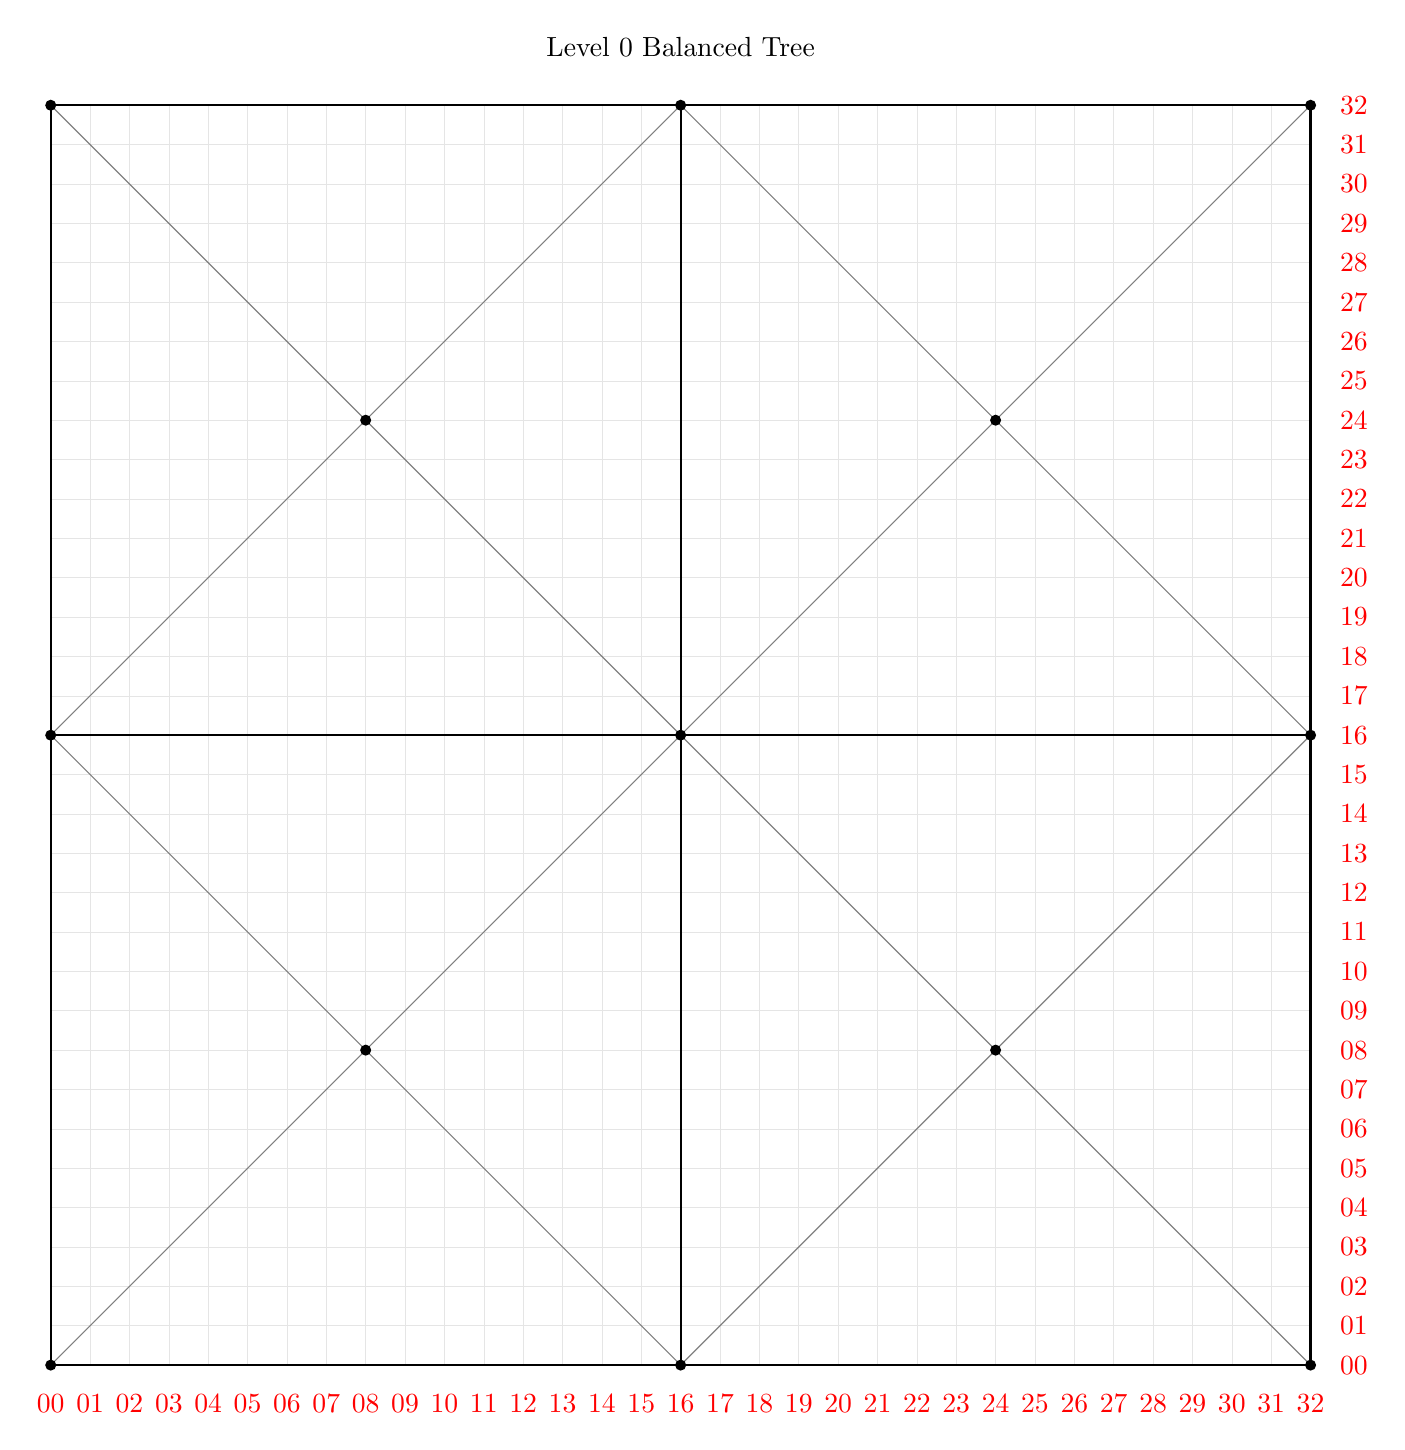
\begin{tikzpicture}[x=0.5cm,y=0.5cm,text centered]

  \node (TOPL) at (16,33) [above,align=center]  {Level 0 Balanced Tree};

  \draw[step=1,black!10,very thin] (0.0,0.0) grid (32.0,32.0);
  \foreach \x in {00,01,02,03,04,05,06,07,08,09,...,32} {
    \node (\x) at (\x,-0.5) [red,below]  {$\x$};
  }
  \foreach \y in {00,01,02,03,04,05,06,07,08,09,...,32} {
    \node (\y) at (32.5,\y) [red,right]  {$\y$};
  }

  \draw[thick] (0,0) rectangle (16,32);
  \draw[thick] (0,16) rectangle (16,32); 
  \draw[thick] (16,0) rectangle (32,16);
  \draw[thick] (16,16) rectangle (32,32);

  \draw[gray] (8,8) -- (0,0);
  \draw[gray] (8,8) -- (16,0);
  \draw[gray] (8,8) -- (16,16);
  \draw[gray] (8,8) -- (0,16);

  \draw[gray] (8,24) -- (0,16);
  \draw[gray] (8,24) -- (16,16);
  \draw[gray] (8,24) -- (16,32);
  \draw[gray] (8,24) -- (0,32);

  \draw[gray] (24,24) -- (16,16);
  \draw[gray] (24,24) -- (32,16);
  \draw[gray] (24,24) -- (32,32);
  \draw[gray] (24,24) -- (16,32);

  \draw[gray] (24,8) -- (16,0);
  \draw[gray] (24,8) -- (32,0);
  \draw[gray] (24,8) -- (32,16);
  \draw[gray] (24,8) -- (16,16);

  \fill (0,0) circle(2pt);
  \fill (0,16) circle(2pt);
  \fill (0,32) circle(2pt);

  \fill (16,0) circle(2pt);
  \fill (16,16) circle(2pt);
  \fill (16,32) circle(2pt);

  \fill (32,0) circle(2pt);
  \fill (32,16) circle(2pt);
  \fill (32,32) circle(2pt);

  \fill (8,8) circle(2pt);
  \fill (8,24) circle(2pt);

  \fill (24,8) circle(2pt);
  \fill (24,24) circle(2pt);

\end{tikzpicture}

\end{document}
